%!TEX TS-program = xelatex
%!TEX encoding = UTF-8 Unicode

\documentclass[12pt]{extarticle}
% extarticle is like article but can handle 8pt, 9pt, 10pt, 11pt, 12pt, 14pt, 17pt, and 20pt text

\def \ititle {Philosophical Psychology}

\def \isubtitle {Lecture 05}

\def \iauthor {Stephen A. Butterfill}
\def \iemail{s.butterfill@warwick.ac.uk}
\date{}

%for strikethrough
\usepackage[normalem]{ulem}

\input{$HOME/latex_imports/preamble_steve_handout}

%\bibpunct{}{}{,}{s}{}{,}  %use superscript TICS style bib
%remove hanging indent for TICS style bib
%TODO doesnt work
\setlength{\bibhang}{0em}
%\setlength{\bibsep}{0.5em}


%itemize bullet should be dash
\renewcommand{\labelitemi}{$-$}

\begin{document}

\begin{multicols*}{3}

\setlength\footnotesep{1em}


\bibliographystyle{newapa} %apalike

%\maketitle
%\tableofcontents




%---------------
%--- start paste




\def \ititle {Lecture 05: The Developmental Origins of Knowledge of Physical Objects}

\begin{center}

{\Large

\textbf{\ititle}

}



\iemail %

\end{center}


‘... ’tis past doubt, that Men have in their Minds several Ideas ...: It is in the first place to be enquired, How he comes by them?’ \citep[p.~104]{Locke:1975qo}.

What is the nature of infants’ earliest cognition of physical objects?
And how do you get from these early forms of cognition to
knowledge of simple facts about particular physical objects?

\section{4- and 5-month-olds can track briefly occluded objects}

\begin{center}
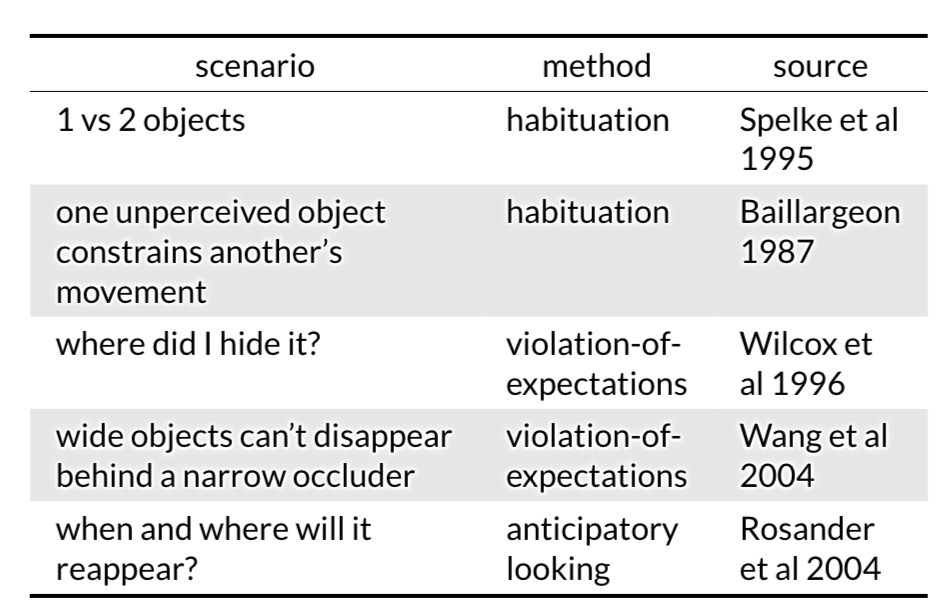
\includegraphics[width=0.3\textwidth]{fig/table1.png}
\end{center}

For a process to \emph{track} an occluded object
is for it to nonaccidentally  depend in some way on
the occluded object’s path.


\section{Core Knowledge}
‘there is a third type of conceptual structure, dubbed “core knowledge” ... that differs systematically from both sensory/perceptual representation[s] ... and ... knowledge.’
\citep[p.~10]{carey:2009_origin}

‘core systems are
largely innate,
encapsulated,
unchanging,
arising from phylogenetically old systems, [and]
built upon the output of innate perceptual analyzers’
\citep[p.~520]{Carey:1996hl}.



\section{The CLSTX Conjecture}

Four- and five-month-olds' abilities to track briefly unperceived objects
are not grounded on belief or knowledge:
instead
they are consequences of the operations of
a system of object indexes.
\citep{Leslie:1998zk,Scholl:1999mi,Carey:2001ue,scholl:2007_objecta,carey:2009_origin}.

An \emph{object index} is ‘a mental token that functions as a
pointer to an object’ \citep[p.\ 11]{Leslie:1998zk}.

The \emph{object-specific preview benefit} is the reduction in time needed to identify that a letter (or other feature) matches a target presented earlier when the letter and target both appear on the same object rather than on different objects.

Object indexes ...
\begin{itemize}
\item guide ongoing action (e.g.~visual tracking, reaching)
\item influence how attention is allocated
\citep{flombaum:2008_attentional}
\item can be assigned in ways incompatible with beliefs and knowledge \citep[e.g.][]{Mitroff:2004pc, mitroff:2007_space}
\item have behavioural  and neural markers, in adults and infants   \citep{richardson:2004_multimodal,kaufman:2005_oscillatory}.
\item are subject to signature limits \citep[pp.~83--87]{carey:2009_origin}
\item sometimes survive occlusion \citep{flombaum:2006_temporal}
\end{itemize}

A \emph{signature limit of a system} is a pattern of behaviour the system exhibits which is both defective given what the system is for and peculiar to that system.


\section{Objects Represented Motorically}
In adults, merely observing a handled object that appears within reach produces brain activity linked to the hand with which it could most readily be grasped \citep{cardellicchio:2011_space}.

Putting a barrier (even a translucent one) between you and a graspable object eliminates or greatly reduces the tendency to represent the object motorically \citep[e.g.][]{costantini:2010_where}.

\emph{Revised CLSTX Conjecture}:
Four- and five-month-olds' abilities to track briefly unperceived objects are also consequences of a further, independent capacity to track physical objects which involves motor representations and processes.

Prediction: When occluders and barriers are deconfounded, infants’ performance is consistent with the Revised CLSTX Conjecture (see \citealp{mccurry:2009_beyond}).


\section{Metacognitive Feelings}
How could the operations of object indexes explain purposive actions like looking longer at one thing than another?

Metacognitive feelings are aspects of the overall phenomenal character of experiences which their subjects take to be informative about things that are only distantly related (if at all) to the things that those experiences intentionally relate the subject to.

Metacognitive feelings can be thought of as sensations in approximately Reid’s sense: they are monadic properties of events, specifically perceptual experiences,
which are individuated by their normal causes
and which alter the overall phenomenal character of those experiences in ways not determined by the experiences’ contents
(so two perceptual experiences can have the same content but distinct sensational properties).

Metacognitive feelings are signs:
they can lead to beliefs only via associations or further beliefs
(\citealp[Essay~II, Chap.~16, p.~228]{Reid:1785cj};
\citealp[Chap.~VI sect.~III, pp.~164–5]{Reid:1785nz}).


\section{Development is Rediscovery}
If core knowledge is a hybrid of object indexes, motor representations and metacognitive feelings,
how do you get from core knowledge to knowledge proper?

\emph{The Assumption of Representational Connections}: the transition involves operations on the contents of core knowledge states, which transform them into (components of) the contents of knowledge states.

Most proposals rely on this assumption, including:
(i) Spelke’s suggestion that mature understanding of objects derives from core knowledge by virtue of core knowledge representations being assembled (\citeyear{Spelke:2000nf}); (ii) claims by Leslie and others that modules provide conceptual identifications of their inputs \citep{Leslie:1988ct}; (iii) Karmiloff-Smith’s representational re-description (\citeyear{Karmiloff-Smith:1992lv}); and (iv) Mandler’s claim that ‘the earliest conceptual functioning consists of a redescription of perceptual structure’ (\citeyear{Mandler:1992vn}).
%\begin{itemize}
%\item assembling core knowledge from different domains \citep{Spelke:2000nf}
%\item modules provide conceptual identifications of their inputs
%\citep{Leslie:1988ct}
%\item representational re-description
%\citep{Karmiloff-Smith:1992lv}
%\item ‘the earliest conceptual functioning consists of a redescription of perceptual structure’ \citep{Mandler:1992vn}
%\end{itemize}

Core knowledge influences actions only, or primarily, via metacognitive feelings, the Assumption of Representational Connections is wrong.

\emph{Alternative assumption}: the transition depends only on the effects of core knowledge states on behaviour, attention, and phenomenology.

Development is rediscovery: the emergence of knowledge involves rediscovering information already encoded as core knowledge.


\footnotesize
\bibliography{$HOME/endnote/phd_biblio}

\end{multicols}

\end{document}
